\documentclass[a4paper]{article}

\usepackage[a4paper, top=8mm, bottom=8mm, left=8mm, right=8mm]{geometry}

\usepackage{polyglossia}
\setdefaultlanguage[babelshorthands=true]{russian}
\setotherlanguage{english}

\usepackage{fontspec}
\setmainfont{FreeSerif}
\newfontfamily{\russianfonttt}[Scale=0.7]{DejaVuSansMono}

\usepackage[tiny, compact]{titlesec}

\usepackage{titling}
\setlength{\droptitle}{-1cm}
\pretitle{\begin{center}\begin{bfseries}\Large}
\posttitle{\par\end{bfseries}\end{center}}
\preauthor{\begin{center}\normalsize}
\postauthor{\par\end{center}\vspace{-1.8cm}}

\usepackage{hyperref}
\usepackage{bookmark}
\usepackage{csquotes}
\usepackage{enumitem}
\usepackage{amsmath}
\usepackage{graphicx}

\title{Реализация свёртки изображений на Python}

\author{Замятина Элла Андреевна}

\date{}

\begin{document}

\maketitle

\begin{flushright}
    Группа: \emph{\enquote{25.Б43-мм}}

    Кафедра: \emph{системного программирования}

    Научный руководитель: \emph{Пономарев Николай Алексеевич}

    Номер семестра практики: \emph{2}
\end{flushright}

\section{Введение}

Свёртка~--- одна из базовых операций в обработке изображений. Она применяется для размытия, повышения резкости, выделения границ и других преобразований. Двумерная свёртка изображения $I$ с ядром $K$ размера $k \times k$ определяется как сумма поэлементных произведений пикселей окна и коэффициентов ядра:
\[
(I * K)[i, j] = \sum_{u=0}^{k-1} \sum_{v=0}^{k-1} I_{\text{pad}}[i+u,\, j+v] \cdot K[u, v],
\]
где $I_{\text{pad}}$~--- изображение после дополнения границ. В работе реализована данная операция на языке Python, проведено тестирование и сравнение производительности с OpenCV и Pillow.

\section{Постановка задачи}

\textbf{Цель работы:} реализовать операцию двумерной свёртки изображений, провести тестирование и сравнить производительность с библиотечными аналогами.

\textbf{Задачи:}
\begin{itemize}
    \item Реализовать функцию свёртки, работающую как с RGB-изображениями, так и с полутоновыми изображениями.
    \item Реализовать четыре режима дополнения границ: \verb|zero|, \verb|edge|, \verb|reflect|, \verb|wrap|.
    \item Подготовить набор из восьми ядер размером $3 \times 3$ и $5 \times 5$.
    \item Написать интеграционные тесты с эталонными изображениями.
    \item Провести сравнительный анализ производительности собственной реализации с OpenCV и Pillow.
\end{itemize}

\section{Реализация}

Проект представляет собой консольное приложение на языке Python. Выбор данного формата обусловлен учебным характером работы: основное внимание уделяется реализации алгоритма свёртки, а не разработке графического интерфейса. При этом сам алгоритм вынесен в отдельный модуль \verb|convolution.py|, который может использоваться как библиотечная функция независимо от интерфейса командной строки. Взаимодействие с пользователем, загрузка и сохранение изображений реализованы в модуле \verb|main.py|. Остальные модули отвечают за отдельные аспекты: \verb|padding.py|~--- дополнение границ, \verb|kernels.py|~--- ядра фильтров, \verb|benchmark.py|~--- визуализация результатов измерений.

\subsection{Загрузка и подготовка изображения}

Изображение загружается с помощью библиотеки Pillow. При наличии флага \verb|--gray| выполняется перевод в полутоновое изображение через встроенный метод \verb|Image.convert("L")|. 
\subsection{Режимы дополнения (padding)}

Поскольку применение ядра к граничным пикселям требует данных за пределами изображения, в модуле \verb|padding.py| реализована функция \verb|apply_padding|, которая дополняет изображение с помощью \verb|np.pad|. Доступны четыре режима:

\begin{itemize}
    \item \textbf{zero}~--- заполнение нулями (\verb|mode="constant"|).
    \item \textbf{edge}~--- копирование крайних пикселей (\verb|mode="edge"|).
    \item \textbf{reflect}~--- зеркальное отражение без дублирования границы (\verb|mode="reflect"|).
    \item \textbf{wrap}~--- циклическое продолжение (\verb|mode="wrap"|).
\end{itemize}

Размер дополнения вычисляется как половина размера ядра: для ядра $3 \times 3$ добавляется по одному пикселю с каждой стороны, для $5 \times 5$~--- по два.

\subsection{Функция свёртки}

Основная функция \verb|apply_convolution| из модуля \verb|convolution.py| принимает изображение в виде массива NumPy, ядро свёртки и режим дополнения. Алгоритм работает следующим образом:

\begin{enumerate}
    \item Если изображение двумерное (полутоновое), оно приводится к трёхмерному виду добавлением оси канала.
    \item Вызывается \verb|apply_padding| для формирования дополненного массива.
    \item Функция \verb|sliding_window_view| из NumPy формирует пятимерный массив, где каждый пространственный пиксель содержит окно размера ядра.
    \item Свёртка вычисляется с помощью функции \verb|np.einsum| и опции \verb|optimize="greedy"|.
    \item Результат ограничивается диапазоном $[0, 255]$ и приводится к типу \verb|uint8|.
\end{enumerate}

В процессе разработки проводилась оптимизация. Начальная версия с тремя вложенными циклами по высоте, ширине и элементам ядра демонстрировала время выполнения около 2200~мс для RGB-изображения $1024 \times 1024$ с ядром $3 \times 3$. Замена внутреннего цикла на \verb|sliding_window_view| с последующим \verb|np.sum| позволила сократить время до приблизительно 110~мс. Итоговая версия с \verb|np.einsum| и \verb|optimize="greedy"| выполняет свёртку за примерно 6~мс. Суммарное ускорение составило более 350 раз.

\subsection{Ядра фильтров}

В словаре \verb|KERNELS| модуля \verb|kernels.py| определены 8 ядер. Для каждого типа доступны версии $3 \times 3$ и $5 \times 5$:

\begin{itemize}
    \item \textbf{identity\_kernel}~--- единичное ядро, не изменяет изображение.
    \item \textbf{box\_blur}~--- равномерное усредняющее ядро (box blur).
    \item \textbf{gaussian}~--- гауссово размытие.
    \item \textbf{sharpen}~--- повышение резкости.
\end{itemize}

Ядра загружаются функцией \verb|get_kernel| по строковому имени.

\subsection{Интерфейс командной строки}

Точка входа в \verb|main.py| использует \verb|argparse|. Поддерживаются аргументы:
\begin{itemize}
    \item \verb|input|, \verb|output|~--- пути ко входному и выходному изображению.
    \item \verb|--kernel|~--- выбор ядра (по умолчанию \verb|blur|).
    \item \verb|--padding|~--- режим дополнения (по умолчанию \verb|zero|).
    \item \verb|--gray|~--- флаг перевода в полутоновое изображение.
\end{itemize}

\section{Тестирование}

Для проверки корректности реализованы интеграционные тесты в файле \verb|tests/test_integration.py| с использованием эталонных изображений. Для каждой комбинации ядра и режима дополнения эталонное изображение было заранее получено с помощью библиотеки OpenCV (\verb|cv2.filter2D|) и сохранено в директории \verb|tests/golden/| в формате PNG. При запуске теста функция \verb|apply_convolution| применяет свёртку к входному изображению, после чего результат поэлементно сравнивается с эталоном с помощью \verb|np.array_equal|, что гарантирует точное совпадение.

\section{Экспериментальное исследование производительности}

Эксперименты проводились на системе со следующими характеристиками:
\textit{процессор} Intel Core i5-5200U, \textit{ОЗУ} 16~ГБ, \textit{ОС} EndeavourOS Linux.

Для измерений использовалась библиотека \verb|pytest-benchmark| (файл \verb|tests/test_benchmark.py|). Сравнивались три реализации:
\begin{itemize}
    \item \textbf{custom}~--- собственная функция \verb|apply_convolution|.
    \item \textbf{opencv}~--- \verb|cv2.filter2D|.
    \item \textbf{pillow}~--- \verb|ImageFilter.Kernel|.
\end{itemize}

Измерения проводились на случайных изображениях размеров $1024 \times 1024$ и $2048 \times 2048$ пикселей в двух цветовых режимах (RGB и полутоновом) для всех 8 ядер. Измерения запускались через pytest с библиотекой \verb|pytest-benchmark|, результаты визуализированы скриптом \verb|benchmark.py| и представлены на рисунке~\ref{fig:bench}.

\begin{figure}[ht]
    \centering
    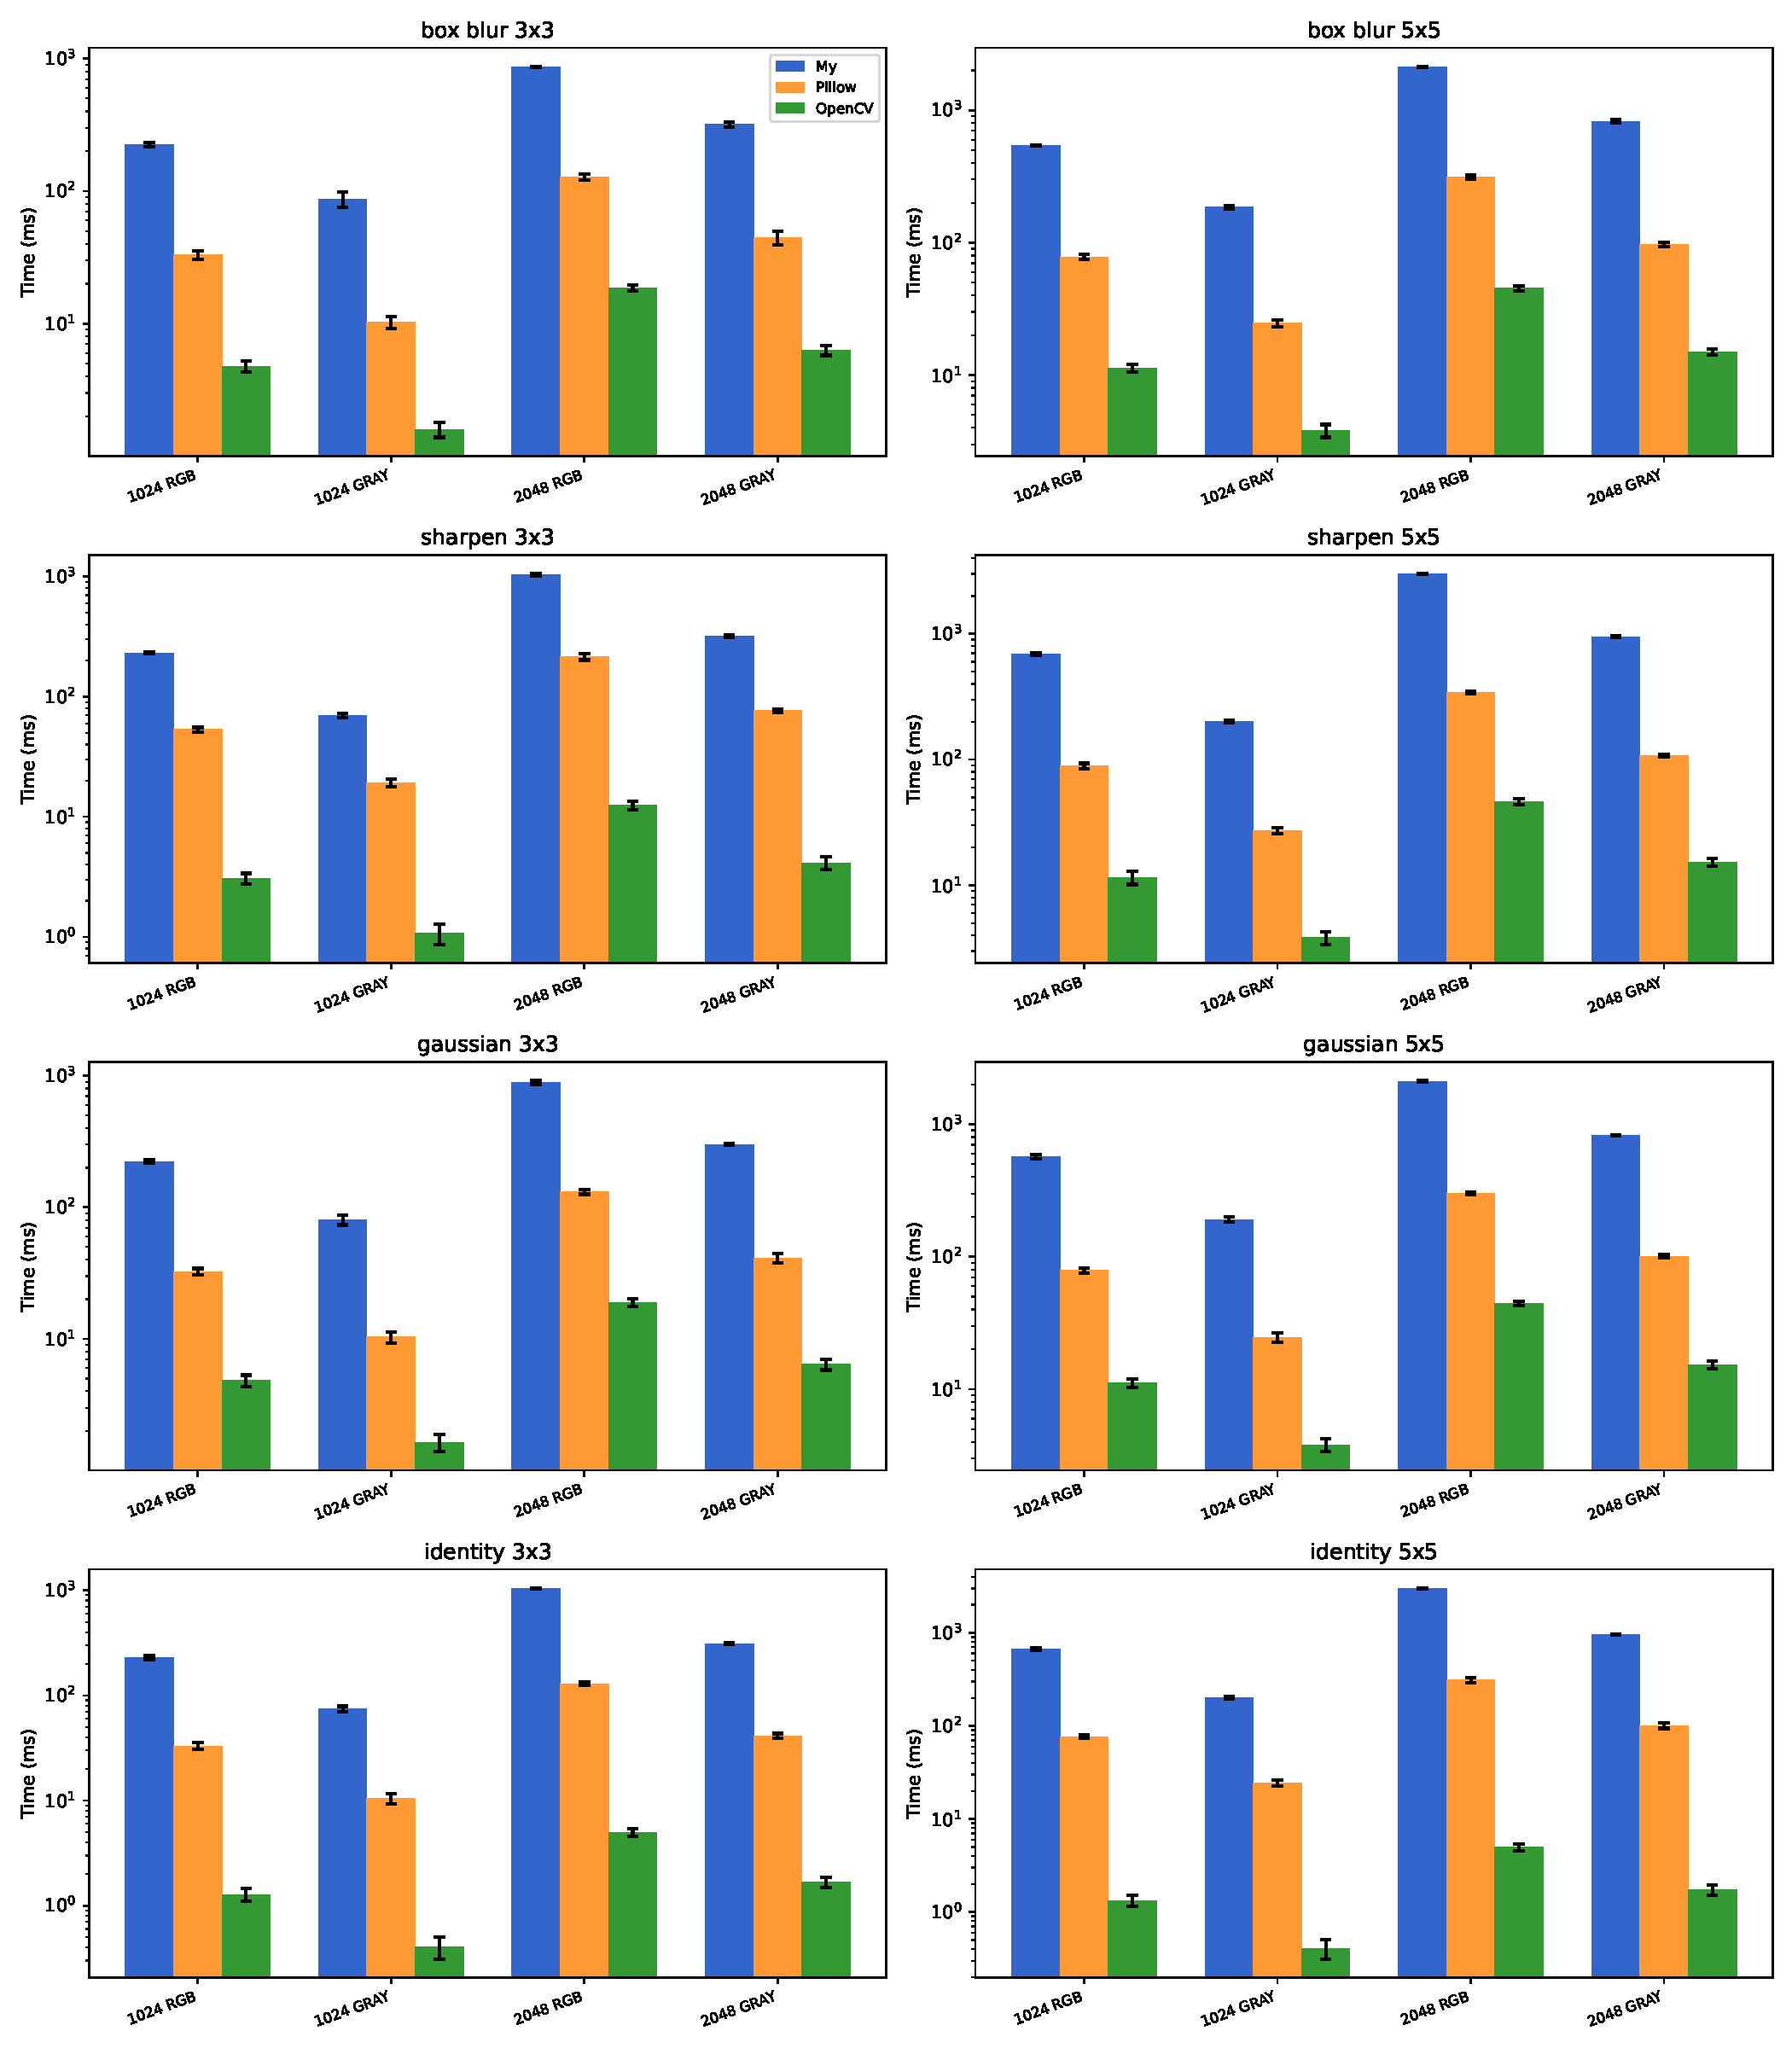
\includegraphics[width=0.825\textwidth]{benchmark.pdf}
    \caption{Сравнение времени выполнения свёртки для трёх реализаций. Ось Y~--- логарифмическая. Планки погрешностей соответствуют стандартному отклонению по 5 запускам.}
    \label{fig:bench}
\end{figure}

OpenCV является наиболее быстрой реализацией для всех конфигураций благодаря низкоуровневым оптимизациям на C++ и SIMD-инструкциям. Pillow показывает промежуточные результаты. Собственная реализация уступает библиотечным, однако после применения \verb|np.einsum| время выполнения существенно сократилось по сравнению с исходной версией. Размер ядра влияет на производительность: для ядер $5 \times 5$ время выполнения в 2--5 раз больше, чем для $3 \times 3$. Обработка полутоновых изображений выполняется быстрее RGB пропорционально числу каналов.

\section{Заключение}

В ходе выполнения работы получены следующие результаты:
\begin{itemize}
    \item Написаны интеграционные тесты на основе эталонных изображений, подтверждающие корректность реализации.
    \item Проведено сравнение производительности с OpenCV и Pillow, показавшее ожидаемое преимущество библиотечных реализаций.
\end{itemize}

Репозиторий с реализацией: \url{https://github.com/ellazamyatina/image_convolution_practice}

\end{document}
